\documentclass[11pt,a4paper]{article}
\usepackage{fontspec}
\usepackage{polyglossia}
\setdefaultlanguage{italian}
\setmainfont{TeX Gyre Termes}
\setmonofont{Latin Modern Mono}[Scale=0.95]
\usepackage[margin=2.6cm,top=2.8cm,bottom=2.8cm]{geometry}
\usepackage{graphicx,booktabs,amsmath,xcolor,listings,fancyhdr,caption,titlesec,microtype,enumitem}
\usepackage{icomma}
\usepackage[hidelinks]{hyperref}
\usepackage{float}
\usepackage[round,authoryear]{natbib}

\definecolor{codebg}{HTML}{F5F5F2}
\definecolor{codekw}{HTML}{1C5CAB}
\definecolor{codecm}{HTML}{6E6D68}
\lstset{language=Python,basicstyle=\ttfamily\small,backgroundcolor=\color{codebg},
  keywordstyle=\color{codekw},commentstyle=\color{codecm}\itshape,
  frame=none,xleftmargin=1em,framexleftmargin=1em,aboveskip=8pt,belowskip=8pt,
  columns=fullflexible,keepspaces=true,showstringspaces=false}

\captionsetup{font={small,it},labelfont={small,it},justification=centering}
\titleformat{\section}{\large\bfseries}{\thesection.}{0.5em}{}
\titleformat{\subsection}{\normalsize\bfseries}{\thesubsection}{0.5em}{}
\titlespacing*{\section}{0pt}{14pt}{6pt}
\titlespacing*{\subsection}{0pt}{10pt}{4pt}
\setlength{\parskip}{5pt}\setlength{\parindent}{0pt}

\pagestyle{fancy}\fancyhf{}
\fancyhead[L]{\small\itshape L'impronta fiscale del Superbonus 110\%}
\fancyhead[R]{\small\itshape Ettore Mancuso}
\fancyfoot[C]{\small\thepage}
\renewcommand{\headrulewidth}{0.4pt}\renewcommand{\footrulewidth}{0.4pt}

\begin{document}
\thispagestyle{empty}
\begin{center}
{\LARGE\bfseries Chi paga il boom delle ristrutturazioni:\\[4pt] l'impronta fiscale del Superbonus 110\%}\\[10pt]
{\large\itshape Un'analisi basata sui dati di adesione, contabilizzazione nel deficit,\\ tempi di impatto sul debito e moltiplicatore che sarebbe servito}\\[22pt]
{\large Ettore Mancuso}\\[1pt]
\href{mailto:ettoremancuso6@gmail.com}{ettoremancuso6@gmail.com}\\[1pt]
Settembre 2026
\end{center}
\vspace{16pt}

\section*{Sommario}
Tra il 2020 e il 2025 l'Italia ha finanziato la ristrutturazione di circa mezzo milione di edifici con il Superbonus 110\%, un credito d'imposta superiore al costo dei lavori e, fino al 2023, liberamente cedibile a terzi. Ho costruito un piccolo dataset con dati ENEA, Istat, Commissione europea e studi empirici recenti, indicando la fonte di ogni numero, e su questo ho svolto quattro esercizi in Python. Il primo ricostruisce l'adesione: gli investimenti certificati sono cresciuti di circa 3,8 miliardi di euro al mese tra metà 2022 e fine 2023, si sono fermati quando è stata eliminata la cessione del credito e hanno raggiunto i 124 miliardi. Il secondo scompone il deficit: nel 2023 i crediti edilizi pesano per circa 4 dei 7,2 punti di PIL di indebitamento netto, e senza di essi il deficit sarebbe rimasto vicino al 3\%. Il terzo usa un modello stilizzato delle compensazioni di cassa per spiegare perché lo stesso costo arriva al debito pubblico anni dopo essere entrato nel deficit: circa il 2\% di PIL all'anno viene assorbito tra il 2024 e il 2026, e il profilo cambia poco se si modificano le ipotesi sulle rate. Il quarto è un'analisi di pareggio. Con le quote di deadweight stimate da Banca d'Italia e MEF (27--38\%), ogni euro di costruzioni aggiuntive avrebbe dovuto generare 1,36--1,60 euro di PIL perché la misura andasse in pari in termini di prodotto, e più di 3 euro perché si ripagasse con il gettito. Lo stimolo ha funzionato, ma è costato molto, e il suo disegno non dava a nessuno un motivo per contenere i prezzi.

\medskip
\textbf{Parole chiave:} politica fiscale, crediti d'imposta, Superbonus, moltiplicatore fiscale, deadweight, debito pubblico, contabilità pubblica, Italia

\textbf{Classificazione JEL:} E62, H24, H62, H63, R31, Q48

\section{Introduzione}
Nel maggio 2020, con il PIL italiano avviato verso un calo dell'8,9\% su base annua, il governo ha introdotto un incentivo alle ristrutturazioni con due obiettivi: rilanciare un settore edile fermo da oltre dieci anni e accelerare la transizione energetica \citep{capone2026}. Il Superbonus 110\% aveva due caratteristiche insolite. Il contributo superava l'intero costo dei lavori, e il credito che ne derivava si poteva cedere a una banca o trasformare in uno sconto immediato in fattura. Nato come misura di un anno, è stato prorogato più volte ed è sopravvissuto a tre governi. Insieme al bonus facciate, il suo costo fiscale complessivo è stimato in circa 220 miliardi di euro, circa 150 in più rispetto alle previsioni iniziali \citep{capone2026}.

Sulla misura esiste già una letteratura ampia. Gli studi controfattuali di Banca d'Italia e MEF stimano quanta parte degli investimenti sia stata davvero aggiuntiva \citep{accetturo2026,mef_wp}; Corsello ed Ercolani ne misurano l'effetto sui costi di costruzione \citep{corsello2024,corsello2025}; le analisi istituzionali ne valutano le conseguenze sui conti pubblici \citep{codogno2024,imf2024}. Io non provo a produrre una nuova stima causale. L'obiettivo è più limitato: mettere i numeri pubblici in un unico dataset riproducibile e applicarci strumenti che si imparano in un corso triennale di economia, cioè le identità della contabilità nazionale, una piccola simulazione e una condizione di pareggio per il moltiplicatore fiscale. Le domande sono tre:

\begin{enumerate}[leftmargin=1.5em,itemsep=2pt]
\item Quanto ha pesato la misura sul deficit, e quanto ha contato il trattamento contabile?
\item Perché il costo arriva al debito pubblico anni dopo essere comparso nel deficit?
\item Data la quota di deadweight stimata, quale moltiplicatore sarebbe servito per andare in pari, o per far sì che la misura si ripagasse da sola?
\end{enumerate}

La sezione~2 descrive il funzionamento della misura, la sezione~3 i dati e i metodi. La sezione~4 presenta i risultati, la~5 li confronta con la letteratura, la~6 ne discute i limiti e la~7 conclude. Figure e tabelle sono prodotte da un notebook Jupyter allegato.

\section{Come funzionava la misura}
L'Italia concede detrazioni per le ristrutturazioni dalla fine degli anni Novanta, con aliquote salite al 65--75\% per gli interventi di efficienza energetica dopo il 2007 \citep{capone2026}. Il Superbonus ha rotto con questa tradizione su due punti. L'aliquota del 110\% copriva tutto il costo dei lavori ammessi più un margine implicito di finanziamento, recuperato in quattro o cinque rate annuali. E il credito era cedibile: una famiglia senza abbastanza imposte da compensare poteva venderlo, e un'impresa poteva applicare lo sconto in fattura e tenersi il credito.

La cessione serviva a includere le famiglie con poca liquidità. L'effetto collaterale è stato eliminare il normale conflitto di interessi tra chi compra e chi vende: un proprietario rimborsato per più dell'intera fattura non ha alcun motivo di trattare sul prezzo. La cedibilità ha cambiato anche la natura statistica del credito. Secondo le regole del \textit{Manual on Government Deficit and Debt} di Eurostat, un credito che si può trasferire o utilizzare indipendentemente dalle imposte dovute dal titolare è un credito d'imposta \textit{pagabile}: va registrato per intero come spesa pubblica nell'anno in cui si fanno i lavori, e non come minore entrata negli anni in cui viene usato \citep{capone2026,istat2023eurostat}. Dal 2022 le regole sono state ristrette più volte; la cessione per i nuovi interventi è stata abolita nel 2023--24 e l'aliquota è scesa al 70\% per il 2024 e al 65\% per il 2025 \citep{capone2026}.

\section{Dati e metodi}
\subsection{Dati}
Non esiste una banca dati unica sulla misura, quindi l'analisi si basa su quattro file raccolti a mano, con la fonte indicata riga per riga (tabella~\ref{tab:data}). I valori sono in euro correnti o in percentuale del PIL. Segnalo due problemi. La serie ENEA cambia definizione nel tempo (interventi ammessi, investimento totale, investimento ammesso a detrazione); il dato di settembre 2021 riguarda solo i lavori conclusi e per questo lo mostro a parte. La serie del deficit combina l'ultima versione Istat disponibile per ogni anno con le prime stime pubblicate per il 2020--2022, così da rendere visibile l'effetto della riclassificazione.

\begin{table}[H]\centering\small
\caption{Dati utilizzati nell'analisi.}\label{tab:data}
\begin{tabular}{p{3.6cm}p{5.0cm}p{5.1cm}}
\toprule
File & Contenuto & Fonti \\
\midrule
\texttt{enea\_takeup.csv} & Investimenti certificati cumulati e numero di edifici, 2021--2025 & Report mensili ENEA, tramite \citet{upb2024}, BUILD UP, Eurofound, Edilportale, BibLus, Teleborsa \\
\texttt{enea\_composition} & Asseverazioni e investimenti per tipo di edificio, 30 settembre 2025 & ENEA tramite \citet{edilportale2025} \\
\texttt{deficit.csv} & Indebitamento netto 2019--2025, prime stime, costo per competenza dei crediti edilizi & Comunicati Istat 2023--2026; \citet{agi2023}; \citet{corsello2025}; \citet{ec2025} \\
\texttt{literature\_estimates} & Stime di adesione e di deadweight & \citet{accetturo2026}; \citet{mef_wp} \\
\bottomrule
\end{tabular}
\end{table}

\subsection{Scomposizione del deficit}
Divido l'indebitamento netto in due parti: il costo per competenza dei crediti edilizi e tutto il resto. Per la componente dei crediti seguo \citet{corsello2025}, che la stimano in quasi l'1\%, il 3\% e il 4\% del PIL nel 2021, 2022 e 2023; il valore 2024 (0,5\%) lo ricavo dalla Commissione europea, secondo cui il calo dei crediti edilizi ha ridotto il deficit di circa 3,5 punti tra il 2023 e il 2024 \citep{ec2025}. Il resto è un residuo contabile e non un controfattuale: senza la misura sarebbero stati diversi anche il PIL e il gettito.

\subsection{Simulazione delle compensazioni di cassa}
Sia $A_t$ l'ammontare di crediti maturati nell'anno $t$ (in percentuale del PIL) e $n_t$ il numero di rate annuali uguali in cui quella annata viene utilizzata, a partire da $t+1$. Il costo di cassa nell'anno $s$, cioè quello che fa salire il fabbisogno e quindi il debito, è
\begin{equation}
C_s=\sum_{t}\frac{A_t}{n_t}\,\mathbf{1}\{\,t< s\le t+n_t\,\}.
\end{equation}
Nello scenario base uso cinque rate per i lavori del 2021, quattro per il 2022--23 e dieci per il 2024, la regola introdotta quell'anno \citep{imf2024}. Tengo fermo il PIL: il modello descrive i tempi, non è una previsione. Riporto qui sotto la funzione completa.

\begin{lstlisting}
def cash_profile(accruals, instalments, start_lag=1, horizon=(2021, 2034)):
    # Ripartisce ogni annata di crediti pagabili in compensazioni annuali uguali.
    # accruals: {anno: % del PIL maturato}; instalments: {anno: numero di rate}
    years = np.arange(horizon[0], horizon[1] + 1)
    cash = pd.Series(0.0, index=years)
    for t, a in accruals.items():
        n = instalments[t]
        for k in range(n):
            s = t + start_lag + k
            if s in cash.index:
                cash[s] += a / n
    return cash
\end{lstlisting}

\subsection{Il moltiplicatore di pareggio}
Siano $s$ il costo fiscale per ogni euro di lavori agevolati, $d$ la quota di deadweight (la spesa agevolata che ci sarebbe stata comunque) e $k$ l'effetto sul PIL di un euro di spesa aggiuntiva in costruzioni, compresi gli effetti indiretti e indotti. Il moltiplicatore implicito sul denaro pubblico è
\begin{equation}
m=\frac{k\,(1-d)}{s}.
\end{equation}
La misura va in pari in termini di prodotto quando $m\ge 1$, e si ripaga da sola quando il gettito aggiuntivo copre il costo, cioè $\tau m\ge1$, dove $\tau$ è il rapporto tra entrate fiscali e PIL. Pongo $s=1$, una media tra il 110\% del Superbonus e il 90\%/60\% del bonus facciate, e $\tau=42,7\%$, la pressione fiscale Istat del 2022 \citep{istat2023conti}. Risolvendo per $k$ si ottengono le due soglie $k^{*}=s/(1-d)$ e $k^{**}=s/[\tau(1-d)]$.

\section{Risultati}
\subsection{L'andamento delle adesioni}
La figura~\ref{fig:takeup} mostra gli investimenti cumulati certificati all'ENEA. Tra luglio 2022 e dicembre 2023 lo stock passa da 40 a 104 miliardi di euro, circa 3,8 miliardi al mese. Dopo l'abolizione della cessione per i nuovi interventi e il taglio dell'aliquota, la crescita scende a circa 0,6 miliardi al mese nel 2025, e a fine 2025 la serie si assesta intorno ai 124 miliardi su 502.544 edifici. A far decollare la misura, secondo me, è stata soprattutto la cedibilità del credito, più dell'aliquota in sé.

\begin{figure}[htbp]\centering
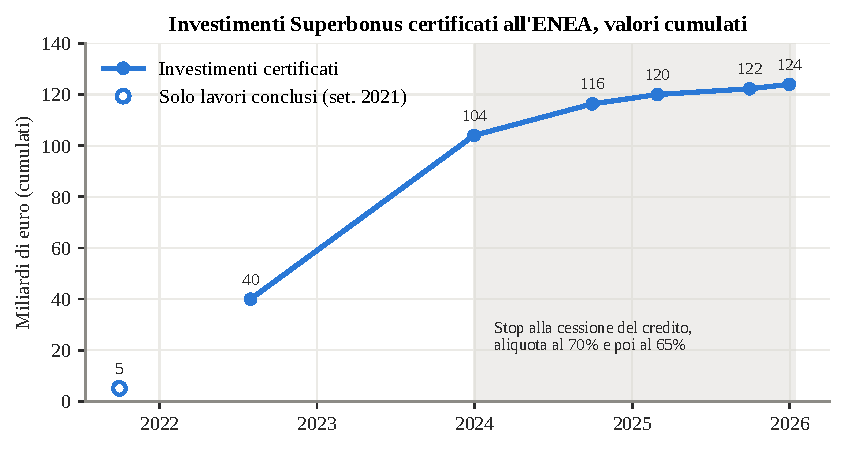
\includegraphics[width=0.86\textwidth]{../figures_it/fig1_takeup.pdf}
\caption{Investimenti Superbonus cumulati certificati all'ENEA. Il punto vuoto misura solo i lavori conclusi e non è direttamente confrontabile con i successivi.}\label{fig:takeup}
\end{figure}

La figura~\ref{fig:comp} confronta, per ciascun tipo di edificio, la quota di asseverazioni con la quota di investimenti. I condomini sono il 28\% delle asseverazioni ma il 68\% degli investimenti, con una media di circa 600.000 euro per asseverazione contro i circa 110.000 delle case unifamiliari. I soldi si sono quindi concentrati in una minoranza di progetti grandi, e questo conta per il discorso distributivo della sezione~5.

\begin{figure}[htbp]\centering
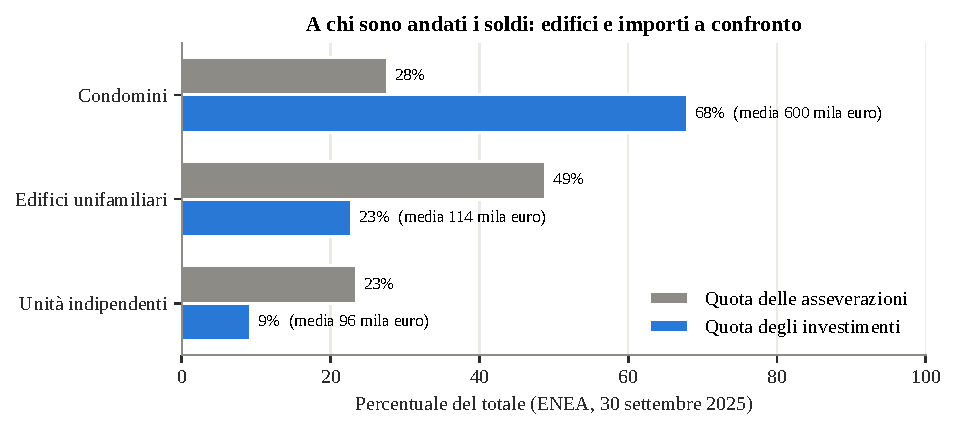
\includegraphics[width=0.86\textwidth]{../figures_it/fig2_composition.pdf}
\caption{Quota di asseverazioni e di investimenti per tipo di edificio, dati ENEA al 30 settembre 2025.}\label{fig:comp}
\end{figure}

\subsection{Il peso sul deficit}
La figura~\ref{fig:deficit} scompone l'indebitamento netto. I rombi arancioni mostrano quanto abbia cambiato le cose la riclassificazione dei crediti come pagabili: il deficit 2021, pubblicato inizialmente al 7,2\% del PIL, oggi è all'8,9\%, e quello 2022 è all'8,1\% contro un obiettivo del 5,6\% \citep{agi2023}. Nel 2023 i crediti edilizi valgono circa 4 dei 7,2 punti di indebitamento netto; il residuo, 3,2\% del PIL, è vicino al valore di riferimento del 3\% previsto dalle regole europee. Il forte miglioramento del 2024, al 3,4\%, si deve in gran parte alla scomparsa meccanica dei crediti e non a una manovra di consolidamento \citep{ec2025}.

\begin{figure}[htbp]\centering
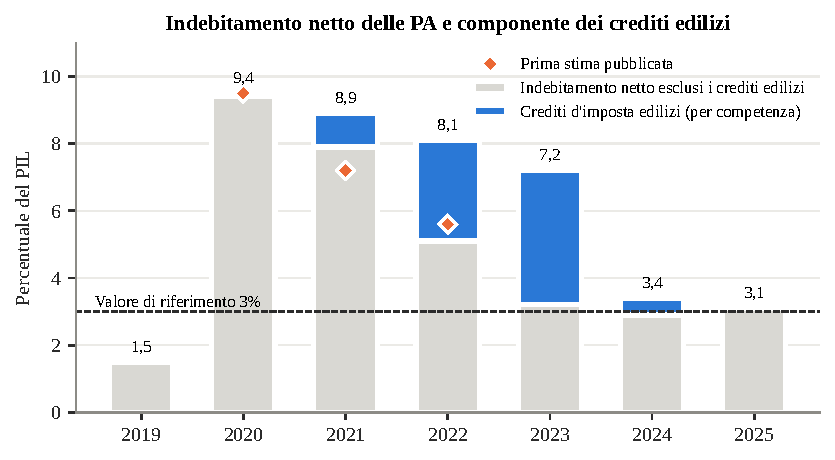
\includegraphics[width=0.86\textwidth]{../figures_it/fig3_deficit.pdf}
\caption{Indebitamento netto delle amministrazioni pubbliche, con il costo per competenza dei crediti d'imposta edilizi e le prime stime pubblicate per il 2020--2022. Il residuo è una scomposizione contabile, non un controfattuale.}\label{fig:deficit}
\end{figure}

\subsection{Dal deficit al debito}
La figura~\ref{fig:cash} riporta i risultati del modello di cassa. Crediti maturati per l'8,5\% del PIL tra il 2021 e il 2024 si traducono in compensazioni di circa il 2\% del PIL all'anno nel 2024--2026, che scendono intorno all'1\% nel 2027 e poi diventano trascurabili. Il deficit migliora quindi prima del debito. Il modello riproduce l'andamento indicato dalle fonti ufficiali: il FMI si aspettava che l'utilizzo dei crediti si concentrasse nel 2024--27 \citep{imf2024}, e l'Istat prevedeva un rapporto debito/PIL in lieve aumento fino al 2026 e in calo dal 2027, man mano che questi effetti si esauriscono \citep{buildnews2024}. Come verifica grossolana, il costo di cassa cumulato 2025--2027 del modello, 5,05 punti di PIL, è dello stesso ordine dei 4,6 punti che una fonte secondaria attribuisce al Rapporto 2025 dell'Ufficio parlamentare di bilancio \citep{liberi2025}.

\begin{figure}[htbp]\centering
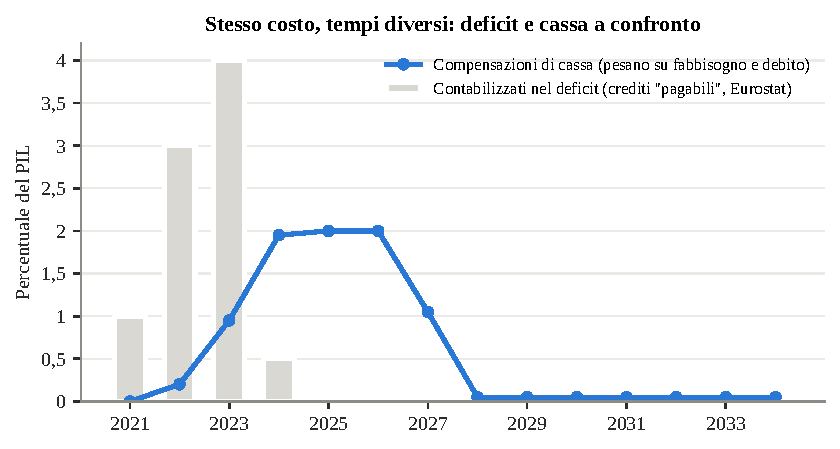
\includegraphics[width=0.86\textwidth]{../figures_it/fig4_cash_sim.pdf}
\caption{Costo per competenza dei crediti edilizi nel deficit e compensazioni di cassa simulate, che fanno salire il fabbisogno. PIL tenuto costante.}\label{fig:cash}
\end{figure}

La tabella~\ref{tab:sens} mette alla prova le ipotesi sulle rate. Il picco cade sempre nel 2025, tra l'1,7 e il 2,1\% del PIL, e il costo cumulato 2025--27 resta tra 4,9 e 5,3 punti. La sensibilità vera riguarda la coda: con cinque rate per tutte le annate, circa 1 punto di PIL arriva al debito dopo il 2027.

\begin{table}[H]\centering\small
\caption{Sensibilità del profilo di cassa alle ipotesi sulle rate (percentuale del PIL).}\label{tab:sens}
\begin{tabular}{lcccc}
\toprule
Scenario & Anno di picco & Picco & Totale 2025--27 & Dopo il 2027 \\
\midrule
Base (rate 5/4/4/10) & 2025 & 2,00 & 5,05 & 0,35 \\
Tutte le annate in 4 rate & 2025 & 2,12 & 5,12 & 0,12 \\
Tutte le annate in 5 rate & 2025 & 1,70 & 4,90 & 1,00 \\
Annata 2024 in 4 rate (senza regola dei 10 anni) & 2025 & 2,08 & 5,28 & 0,12 \\
\bottomrule
\end{tabular}
\end{table}

\subsection{Il moltiplicatore che sarebbe servito}
I due studi controfattuali disponibili implicano quote di deadweight del 26,5\% (45 miliardi su 170, Banca d'Italia) e del 37,6\% (70 su 186, MEF). La figura~\ref{fig:mult} mostra il moltiplicatore implicito $m$ al variare del deadweight e dell'effetto $k$ della spesa aggiuntiva. Con la stima della Banca d'Italia, la misura va in pari solo se ogni euro di costruzioni aggiuntive ha prodotto almeno 1,36 euro di PIL; con quella del MEF la soglia sale a 1,60. Sostenere che la misura si ripaghi con il maggior gettito richiede $m\ge 2,34$, cioè un $k$ superiore rispettivamente a 3,19 e 3,76.

\begin{figure}[htbp]\centering
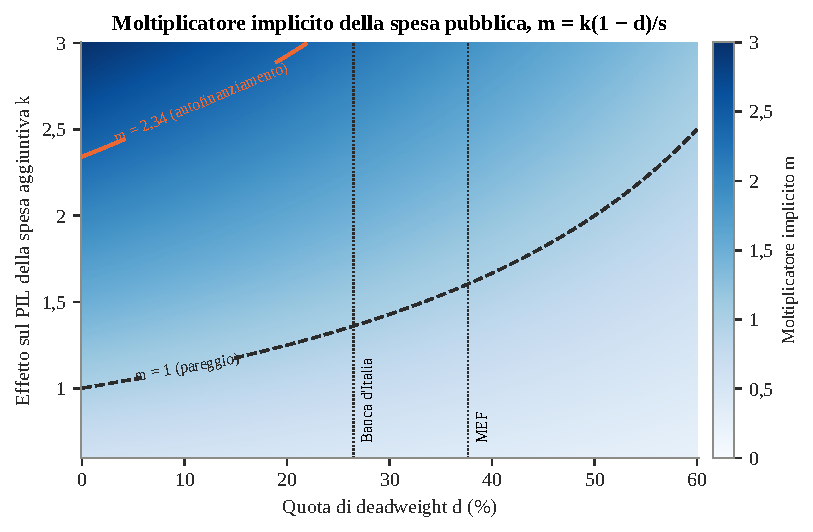
\includegraphics[width=0.84\textwidth]{../figures_it/fig5_multiplier.pdf}
\caption{Moltiplicatore implicito sul denaro pubblico in funzione della quota di deadweight e dell'effetto sul PIL della spesa aggiuntiva, con $s=1$. Curva tratteggiata: pareggio in termini di prodotto; curva continua: autofinanziamento con pressione fiscale al 42,7\%. Le linee punteggiate indicano le due stime di deadweight.}\label{fig:mult}
\end{figure}

La stessa Banca d'Italia stima un moltiplicatore ``di poco inferiore a uno'' \citep{accetturo2026}. Letto con questo schema, equivale a dire che $k$ era sotto 1,35 circa, e l'autofinanziamento resta lontanissimo.

\subsection{Gli effetti sui prezzi}
Un contributo che copre più dell'intera fattura indebolisce anche il segnale di prezzo. Corsello ed Ercolani stimano che il Superbonus spieghi circa 7 dei circa 13 punti di crescita dell'indice Istat dei costi di costruzione tra settembre 2021 e dicembre 2023, quindi più o meno metà \citep{corsello2024,corsello2025}. La figura~\ref{fig:costs} mostra la ripartizione. Una parte del contributo è finita in prezzi più alti pagati ai fornitori a monte, invece di trasformarsi in ristrutturazioni aggiuntive.

\begin{figure}[htbp]\centering
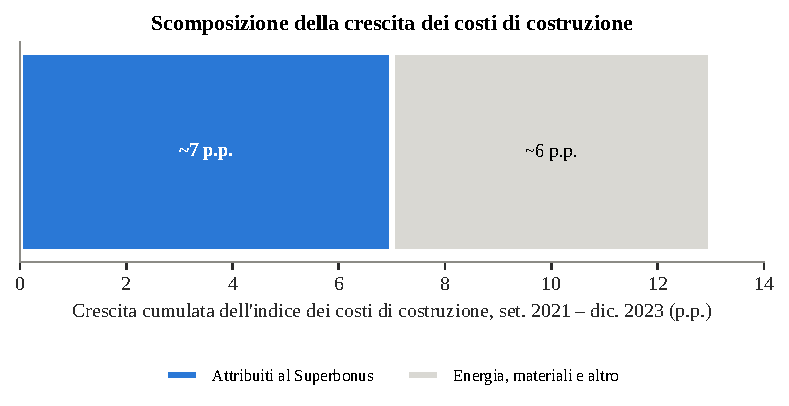
\includegraphics[width=0.84\textwidth]{../figures_it/fig6_costs.pdf}
\caption{Scomposizione della crescita dei costi di costruzione, settembre 2021 -- dicembre 2023, sulla base di \citet{corsello2025}.}\label{fig:costs}
\end{figure}

\section{Il confronto con la letteratura}
La tabella~\ref{tab:lit} mette questi risultati accanto alle stime esistenti, e vanno nella stessa direzione. L'attività è aumentata davvero. Secondo la Banca d'Italia la misura spiega tutta la crescita del valore aggiunto delle costruzioni tra il 2019 e il 2023 \citep{accetturo2026}, e il MEF stima circa 116 miliardi di investimenti residenziali aggiuntivi \citep{mef_wp}. Ma l'Italia ha pagato molto per quello stimolo. Le stime che riportano grandi guadagni di prodotto, come i 124 miliardi e i 634.000 posti di lavoro calcolati da Nomisma, di solito non considerano né il deadweight né il costo del finanziamento \citep{codogno2024}.

\begin{table}[H]\centering\small
\caption{Alcune stime dell'impatto economico del Superbonus.}\label{tab:lit}
\begin{tabular}{p{4.1cm}p{3.4cm}p{6.3cm}}
\toprule
Fonte & Tipo & Risultato principale \\
\midrule
Nomisma, tramite \citet{codogno2024} & Commissionato dal settore & +124 mld di PIL, +634 mila occupati; nessun controfattuale \\
\citet{accetturo2026} & Rivista con referaggio & Deadweight $>$25\% ($>$45 mld); moltiplicatore poco sotto 1 \\
\citet{mef_wp} & Working paper del MEF & $\approx$116 mld di investimenti aggiuntivi; $\approx$70 mld di deadweight \\
\citet{ocpi2023} & Osservatorio universitario & Effetto cumulato sul PIL reale $\approx$1,4\% \\
\citet{capone2026} & Capitolo con referaggio & Quasi tutti i moltiplicatori istituzionali sotto 1; solo quello Istat vicino a 1 \\
Questo lavoro & Esercizio di replica & Pareggio con $k\ge$1,36--1,60; autofinanziamento con $k\ge$3,2--3,8 \\
\bottomrule
\end{tabular}
\end{table}

Due costi non compaiono nei grafici. Il primo sono le frodi: i crediti cedibili si potevano generare per lavori inesistenti e poi rivendere. A dicembre 2025 la Guardia di Finanza riportava oltre 9,3 miliardi di euro di crediti edilizi ed energetici inesistenti sotto sequestro \citep{sky2025}. Il secondo è la distribuzione. La concentrazione degli investimenti nei grandi condomini (figura~\ref{fig:comp}) ne è un indizio. L'Ufficio parlamentare di bilancio ha parlato di un trasferimento dalla generalità dei contribuenti ai proprietari con redditi più alti, e solo il 2\% circa delle risorse è andato all'edilizia popolare \citep{capone2026}. Anche i contributi antisismici si sono in parte capitalizzati nei prezzi delle case, a vantaggio di chi era già proprietario \citep{crispino2025}.

Poi c'è il problema dei tempi. Nella recessione del 2020, con un settore edile pieno di capacità inutilizzata, la misura aveva senso. Nel 2022--23 molto meno, perché si contendeva le stesse imprese e gli stessi lavoratori con il PNRR \citep{codogno2024}. Uno strumento anticiclico prorogato in piena ripresa finisce per diventare prociclico.

\section{Limiti}
Gli esercizi sono descrittivi e volutamente semplici. La scomposizione del deficit sottrae i crediti in modo meccanico e ignora il loro effetto su PIL e gettito. Il modello di cassa tiene fermo il PIL, assume che i titolari usino i crediti appena possibile e non considera il successivo frazionamento di alcune rate: i suoi numeri descrivono i tempi, non prevedono il debito. L'analisi di pareggio dipende da un'aliquota media ipotizzata e da stime di deadweight che vengono da studi con controllo sintetico, sensibili alla scelta dei paesi di confronto. Infine, la serie ENEA cambia definizione nel tempo e diversi valori sono presi da articoli di stampa che riportano dati ufficiali, non dai documenti originali. Le due estensioni più utili sarebbero ricostruire la serie delle adesioni dai report mensili ENEA e stimare $k$ direttamente con le tavole input-output.

\section{Conclusioni e indicazioni di policy}
Il Superbonus ha fatto crescere l'edilizia a un costo molto alto. Il suo costo per competenza spiega gran parte del deficit italiano nel 2022--23, e un semplice modello di cassa mostra perché il conto arriva al debito pubblico anni dopo, a circa il 2\% del PIL all'anno nel 2024--26. Con il deadweight stimato da Banca d'Italia e MEF, la misura sarebbe andata in pari solo se ogni euro di costruzioni aggiuntive avesse prodotto più di 1,36--1,60 euro di PIL, e si sarebbe ripagata solo con un moltiplicatore sopra 2,3. Nessuna stima disponibile ci si avvicina.

Per come la vedo io, l'obiettivo era giusto e lo strumento sbagliato. Le politiche future per la casa possono tenere gli obiettivi di efficienza energetica e sicurezza sismica senza ripetere gli errori del Superbonus: lasciare una quota a carico del beneficiario, così che il prezzo gli interessi; commisurare il sostegno al risparmio energetico atteso e al reddito; affiancare alle detrazioni contributi diretti e accesso al credito; fissare un tetto di spesa con una copertura individuata \citep{deblasio2024}.

\medskip
\textit{Dati e codice: \href{https://github.com/ettoremancuso/superbonus-fiscal-footprint}{github.com/ettoremancuso/superbonus-fiscal-footprint}.}

\renewcommand{\refname}{Riferimenti bibliografici}
\begin{thebibliography}{99}\small\setlength{\itemsep}{2pt}
\bibitem[Accetturo et al.(2026)]{accetturo2026} Accetturo, A., Olivieri, E. e Renzi, F. (2026). Incentives for dwelling renovations: evidence from a large fiscal programme. \textit{Fiscal Studies}, 47(1), 69--87. Versione precedente: Banca d'Italia, Questioni di Economia e Finanza n.~860 (2024).
\bibitem[AGI(2023)]{agi2023} AGI (2023). Effetto superbonus sui conti pubblici. \textit{Agenzia Italia}, 1 marzo 2023.
\bibitem[BuildNews(2024)]{buildnews2024} BuildNews (2024). Superbonus e DEF 2024, l'audizione dell'Istat. 30 aprile 2024.
\bibitem[Capone e Stagnaro(2026)]{capone2026} Capone, L. e Stagnaro, C. (2026). Italy's Superbonus and the capture of climate policy by Modern Monetary Theory. In Henrekson, M., Sandström, C. e Stenkula, M. (a cura di), \textit{A Green Entrepreneurial State?}, 241--255. Springer, Cham.
\bibitem[Codogno(2024)]{codogno2024} Codogno, L. (2024). Italy's Superbonus 110\%: messing up with demand stimulus and the need to reinvent fiscal policy. IMK Study n.~93, Hans-Böckler-Stiftung.
\bibitem[Corsello e Ercolani(2024)]{corsello2024} Corsello, F. e Ercolani, V. (2024). The role of the Superbonus in the growth of Italian construction costs. Banca d'Italia, Questioni di Economia e Finanza n.~903.
\bibitem[Corsello e Ercolani(2025)]{corsello2025} Corsello, F. e Ercolani, V. (2025). The impact of the Superbonus on Italian construction costs. \textit{VoxEU/CEPR}, 9 febbraio 2025.
\bibitem[Consiglio UE(2025)]{ec2025} Consiglio dell'Unione europea (2025). Country Report Italy 2025, doc. ST 9846/25 ADD 1. Bruxelles.
\bibitem[Crispino e Loberto(2025)]{crispino2025} Crispino, M. e Loberto, M. (2025). Bridging policy and prices: causal evidence of housing renovation subsidies on property values in Italy. \textit{Regional Science and Urban Economics}, 112, 104095.
\bibitem[de Blasio et al.(2024)]{deblasio2024} de Blasio, G. et al. (2024). Improving the energy efficiency of homes in Italy: the state of the art and some considerations for public intervention. Banca d'Italia, Questioni di Economia e Finanza n.~845.
\bibitem[Edilportale(2025)]{edilportale2025} Edilportale (2025). Superbonus: superati i 127 miliardi di detrazioni maturate. 22 ottobre 2025.
\bibitem[FMI(2024)]{imf2024} Fondo monetario internazionale (2024). Italy: 2024 Article IV Consultation. IMF Country Report n.~24/240.
\bibitem[Istat(2023a)]{istat2023conti} Istat (2023a). Conti economici nazionali, anni 2020--2022. Comunicato stampa, 22 settembre 2023.
\bibitem[Istat(2023b)]{istat2023eurostat} Istat (2023b). Superbonus, il parere Eurostat. Nota per la stampa, 26 settembre 2023.
\bibitem[Liberi oltre le illusioni(2025)]{liberi2025} Liberi oltre le illusioni (2025). Superbonus: cosa dice realmente il Rapporto UPB 2025? 23 giugno 2025.
\bibitem[MEF(s.d.)]{mef_wp} Ministero dell'Economia e delle Finanze, Dipartimento del Tesoro (s.d.). The effects of tax incentives for dwelling renovations: the case of Italy. Working Paper, Roma.
\bibitem[OCPI(2023)]{ocpi2023} Osservatorio sui Conti Pubblici Italiani (2023). Gli effetti del superbonus 110\% sull'economia e sul bilancio pubblico. Università Cattolica del Sacro Cuore.
\bibitem[Sky TG24(2025)]{sky2025} Sky TG24 (2025). Frodi Superbonus, sequestrati 9,3 mld per finti crediti. 11 dicembre 2025.
\bibitem[UPB(2024)]{upb2024} Ufficio parlamentare di bilancio (2024). Audizione sul Documento di economia e finanza 2024. 22 aprile 2024.
\end{thebibliography}
\end{document}
